\documentclass{NSF}
\usepackage{amssymb}
\usepackage{amsmath}
\usepackage{graphicx}
\graphicspath{ {images/} }


\begin{document}
\author{Myunggun Seo,  Guyu Fan, and Nischal Mainali (Professor: Saurabh Ray)}
\date{December 15, 2018}
\title{Computer Science Capstone Progress Report: Lifting Squares to a Half-space, a Specific Case of Lifting Pseudo-disks}
{\let\newpage\relax\maketitle}

\section{Abstract}
% Your short version of your proposal goes here

\tableofcontents

\section{Introduction}
\subsection{General Case of Pseudo-disks}
The problem that we tackle is a specific case of an unsolved problem in computational geometry: 

Given a set of pseudo-disks $\{D_i\}$ and points $\{P_j\}$ in $\mathbb{R}^2$ in arbitrary positions, (1) determine the existence of a mapping from the pseudo-disks and points to a set of half-spaces $\{H_i\}$ and points $\{Q_j\}$ in $\mathbb{R}^3$ such that the membership of point $P_j$ in a pseudo-disk $D_i$ is preserved with point $Q_j$ in $H_i$ (2) describe the mapping. 

Because shapes in $\mathbb{R}^2$ are mapped to a higher dimension $\mathbb{R}^3$, we will call this problem "lifting."

This is one of a class of mapping methods in Combinatorial Geometry which proved useful because such mappings provide another representation and thus new properties of a geometric problem. Such new properties are used often in cases such as finding lower bounds on $\epsilon$-nets or in Kernel Trick in Machine Learning. 

Although there are specific cases of pseudo-disks such as circles (?) (and anything else? ovals? parabolas? all conic sections?) where this mapping exist and described algebraically, it is not known whether there is such a mapping for other seemingly simple cases like rectangles or squares. 

\subsection{Case of Squares of Equal Size}
Problem statement: Given a set of squares of  $\{S_i\}$ and points $\{P_j\}$ in $\mathbb{R}^2$ in arbitrary positions, is there a mapping from the squares and points to a set of half-spaces $\{H_i\}$ and points $\{Q_j\}$ in $R^3$ such that the membership of point $P_j$ in a square $S_i$ is preserved with point $Q_j$ in $H_i$? If there is, what is the mapping? 

\section{Problems Related to Pseudo-disk Lifting Problem}
\subsection{Solution: Lifting disks of equal radii to half-spaces}
There is an algebraic lifting from disks to half-spaces. Point $(\alpha,\beta)$ is lifted to $(\alpha,\beta,\alpha^2+\beta^2-r^2)$, and disk $(x-a)^2+(y-b)^2\leq r^2$ is lifted to $-2ax -2by + z + (a^2+b^2) \leq 0$ by substituting  $x^2+y^2-r^2$ with $z$. 
\begin{align*}
(\alpha,\beta) & \mapsto (\alpha,\beta,\alpha^2+\beta^2-r^2) \\
(x-a)^2+(y-b)^2\leq r^2 & \mapsto -2ax -2by + z + (a^2+b^2) \leq 0
\end{align*}

The limitation of this method is that it is only possible for disks of equal radii since all points in $\mathbb{R}^2$ can only map to the same point in $\mathbb{R}^3$ which will be defined by the radius $r$.

\subsection{Solution: Lifting disks of varying radii to half-spaces}
Using a similar approach as the above problem, Point $(\alpha,\beta)$ is lifted to $(\alpha,\beta,\alpha^2+\beta^2)$, and disk $(x-a)^2+(y-b)^2\leq r^2$ is lifted to $-2ax -2by + z + (a^2+b^2-r^2) \leq 0$ by substituting  $x^2+y^2$ with $z$. 
\begin{align*}
(\alpha,\beta) & \mapsto (\alpha,\beta,\alpha^2+\beta^2) \\
(x-a)^2+(y-b)^2\leq r^2 & \mapsto -2ax -2by + z + (a^2+b^2-r^2) \leq 0
\end{align*}

\subsection{Idea: Straightening pseudo-disks to disks}
If there is a way to "straighten," or map, a set of general pseudo-disks to disks, then there must be a way to lift any pseudo-disk to a half-space by straightening the pseudo-disks to disks and lifting the produced disks.

\subsection{Similar: Straightening pseudo-lines to lines}
A similar problem to straightening pseudo-disks to disks is straightening pseudo-lines. Pseudo-lines are a set of curves that intersect one another at most once. This property derives from that of lines. The problem is:  given a set of $n$ pseudo-lines, find a positioning of $n$ lines so that the vertical order of the lines match that of the pseudo-lines. This is not always possible to do. (? counter example)

\subsection{Idea: Lifting pseudo-disks to a polytope}
We can see a pseudo-disk as an (infinite) intersection and complements of circles of varying radii. Assuming we can lift disks of varying radii to $\mathbb{R}^3$, the geometry lifted to $\mathbb{R}^3$  from a pseudo-disk can be seen as the intersection and complements of each half-space resulting from lifting the subordinate circles. However, the limitation of this method is that it does not produce half-spaces but produces polytopes which may or may not be convex.




\section{Problems Related to Square Lifting Problem}

\subsection{Case of lifting axis-parallel non-piercing rectangles to half-spaces}
For any pair of axis-parallel non-piercing rectangles, there exist three cases of their positioning:
\begin{enumerate}
\item two disjoint rectangles, without any intersections
\item one rectangle has two corners of the other rectangle inside it
\item each rectangle has a corner in the inside of each other
\item (?) one is completely inside the other
\end{enumerate}
(?) My notes suggest that this can be done in $O(n\log^2{n})$
(?) In the following lines it also suggests that rectangles are defined by two inequalities ($a\leq x \leq b$ and $c \leq y \leq d$ which is one more than what defines a half-space so it is impossible?

\subsection{Solution for lifting rectangles that are fixed to the $x$,$y$-axes to a half-space}
These rectangles are hinged at the origin. For positive $a,b$ values, a rectangle are defined by two inequalities: 
\begin{equation}\label{origin-hinged-1}
0 \leq x \leq a,\  0\leq \  y \leq b
\end{equation}
Since a half-space is defined by just one inequality, we would like to combine the two inequalities into one: 
\begin{equation}\label{origin-hinged-2}
\frac{x}{a} + \frac{y}{b} \leq 2
\end{equation}
Now, \eqref{origin-hinged-1} implies \eqref{origin-hinged-2} but \eqref{origin-hinged-2}  may not imply \eqref{origin-hinged-1}. For \eqref{origin-hinged-2} to imply \eqref{origin-hinged-2}, the values of $x$ and $y$ must satisfy the following: if either $\frac{x}{a}$ or $\frac{y}{b}$ is greater than 1, it should be greater than 2. This means that if $\frac{x}{a}+\frac{y}{b}$  is less than 2, both of its terms are less than 1.

We fulfill the requirement by applying "exponential stretching" on the given set of finite points and rectangles in both $x$ and $y$ directions so that $\frac{x}{a} \geq 2$  for points of which the $x$ coordinate lies beyond the line $x=a$ and $\frac{y}{b} \geq 2$ for points of which the y coordinate lies beyond the line $y=b$.  (?need polishing?)

Then, the inequality \eqref{origin-hinged-2} represents a half-space in $\mathbb{R}^3$. This solution provides a minimum bound on the feasibility of lifting squares or rectangles in general.



\subsection{Solution for lifting rectangles that are fixed to the $x$-axis to a half-space }
In order to update the minimum bound, consider a set of points and rectangles in $\mathbb{R}^2$, each defined by the constraints

\begin{align*}
    \text{point:}& \ x \in \mathbb{R},\  z \geq 0 \\
    \text{rectangle:}& \ x_i \leq x \leq x_j,\ 0 \leq z \leq c
\end{align*}

We'll call such a rectangle a "building," and the two lines $x=x_i$ and $x=x_j$ "walls."
We would like to 
Using ideas from exponential stretching, first sort the $x$ coordinates of all points and all walls together and incrementally assign an integer index to each of them. Stretch out the coordinates of points and walls along the $x$-axis using a steep convex function such as $f(x)=2^x$. 
(? how steep should it be?)
The $i$th $x$ coordinate, be it of a point or a wall, will be mapped to a point in $\mathbb{R}^2$
\begin{equation}
	x_i \mapsto (i, f(i))
\end{equation}
so that if $x_k \in [x_i,x_j]$(ie. the $k$th point is within the walls $x_i,x_j$ of a building), then $l_{ij}(x_k) < 0 $, where $l_{ij}$ for the rectangle with walls  $i$th and $j$th vertical lines is defined as

\begin{equation*}
    l_{ij}(x_k) = [f(k) - f(i)] -[\frac{f(j)-f(i)}{j-i}(k - i)]
\end{equation*}
When $l_{ij}=0$, 

(? why do we need steep functions)
A building's two constraints are respectively changed to 

\begin{equation}\label{x-axis-hinged-separate}
    l_{ij}(x) \leq 0, \ \frac{z}{c} \leq 1
\end{equation}


We need to combine these two inequalities into a single inequality that defines a half-space in $\mathbb{R}^3$. 
The two constraints \eqref{x-axis-hinged-separate} imply the following inequality:
\begin{equation}\label{x-axis-hinged-added}
    l_{ij}(x) + \frac{z}{c} \leq 1 
\end{equation}
To make the converse true, ????
\begin{equation}
	\frac{l_{ij}(x,y)}{\epsilon} + \frac{z}{c} \leq 1
\end{equation}


\subsection{Ideas for mapping squares to disks}
It is enough to find a mapping from a square to disks that preserves point memberships to show that squares can be lifted to half-spaces. Since lifting disks of varying centers and is possible,  The squares to disks and then lift the disks to half-spaces

\subsection{Ideas for mapping disks to squares}

\subsection{Computational approach using Convex Optimization software}

\section{Acknowledgement}


\section{Appendix: Definitions}
\begin{enumerate}
\item A geometric shape is \textbf{axis-parallel} if it is parallel or aligned with a coordinate axis.
\item A \textbf{half-space} in $\mathbb{R}^3$ is either of the two parts separated by a plane. In general, a half-space is either of the two parts divided by a hyperplane in a $\mathbb{R}^k$.
\item \textbf{Helly's theorem} for the Euclidean plane states that if a family of convex sets has a nonempty intersection for every triple of sets, then the whole family has a nonempty intersection. (Wikipedia)
\item \textbf{Membership} of a point and a region is a binary flag that signifies whether the point is inside the region or not.
\item In  $\mathbb{R}^2$, a Jordan curve is \textbf{piercing} another shape if a curve connecting any two points inside the shape must cross the Jordan curve at least twice if the curve lies in the interior of the shape.
\item \textbf{Pseudo-disks} are a set of closed Jordan curves in $\mathbb{R}^2$ in which any pair of pseudo-disks intersect at maximum two places and do not intersect one another. This property is derived from disks in $\mathbb{R}^2$. (?) Can they be inside one another?
\item \textbf{Pseudo-lines} are a set of curves that intersect one another at most once. This property derives from that of lines.
\item 

\end{enumerate}

\subsection{Hypergraphs}



For this research we consider \textbf{undirected graphs} where the order of vertices in an edge does not matter, ie. $e = (v,w) = (w,v)$ for $e$ in $E$ of graph $G = (V, E)$. $G' = (V', E')$ is a \textbf{subgraph} of graph $G = (V, E)$ if $V' \subseteq V$ and $E' \subseteq E$. Also, $G'$ is the vertex-induced subgraph (\textbf{induced subgraph}) of $G$ if $E' = E \cap (V' \times V') $. Verbally, an induced subgraph of a graph is a subgraph that has all of the edges of the original graph that connects each and every vertex in the subgraph.   \\



A \textbf{hypergraph} $H = (V, E)$ consists of the base set $V$, called hypervertices and consisting of vertices and a set $E$, called hyperedges. Hypervertices are the equivalent of a graph's vertex in a hypergraph. The set $E$ is a subset of the powerset of $V \times V$. In other words $E$ contains some subsets of $V$. Formally, $E \subseteq \mathcal{P}(V)\backslash\emptyset$ where $\mathcal{P}(V)$ is the powerset of $V$. \\

The difference between a graph and a hypergraph is that a graph's edges connect two vertices each. Geometrically, an edge can be drawn as an edge but we can see also the edge as a set of two vertices. In a hypergraph, we expand the definition of an edge as a set of any positive number of vertices. The notion of vertices remain the same in hypergraphs.\\

% \subparagraph{Representations of Hypergraphs} 
There are multiple ways to represent a hypergraph. Having multiple representations is useful in thinking creatively from multiple perspectives. As such, different representations have been used to derive proofs and explanations for support graphs because each depiction has a relationship with the support graph. Here we discuss a few.

\begin{figure}[ht]
\centering
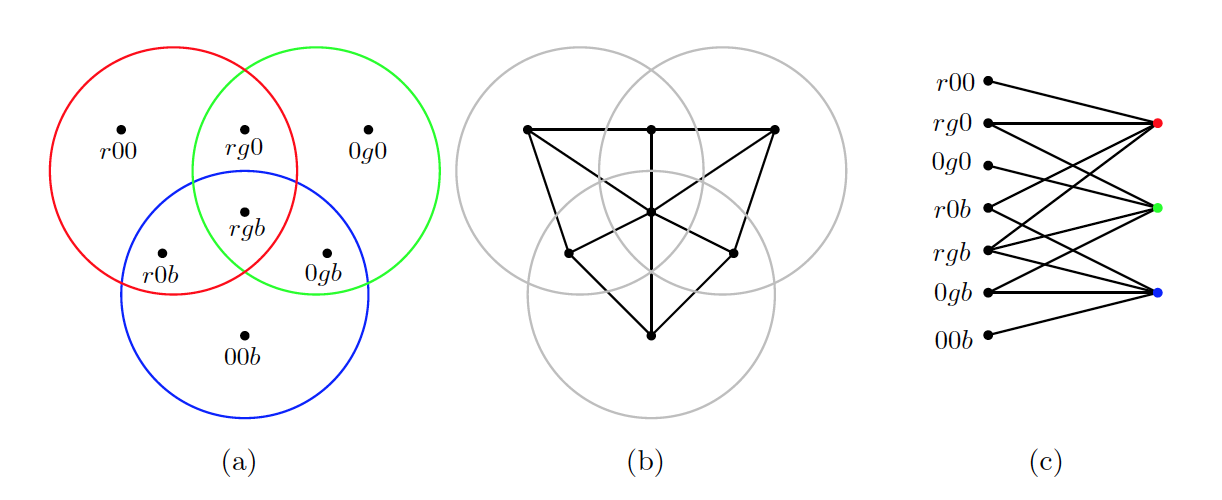
\includegraphics[width=\textwidth]{diagram1}
\caption{Three different representations of hypergraphs: (a) an Euler Diagram of a hypergraph where each Jordan curve represents a hyperedge. For this instance, it is identical to the Venn Diagram (b) the dual of the Euler Diagram which is always a support, and (c) the incidence graph which is a bipartite graph of the vertices on one side and the hyperedges on the other. (Source: Bruckdorfer \cite{tubingen2016})}
\end{figure}

\subparagraph{Euler Diagram}
In an Euler diagram, each hypervertex is shown as a point in the plane and each hyperedge is drawn as a simple closed Jordan curve that encloses all the hypervertices that the hyperedge contains. Figure 1.a depicts an Euler diagram representation of the hypergraph with $V = \{r00, rg0, 0g0, r0b, rgb, 0gb, 00b\}$ and $E = \{  \{r00,rg0,rgb,r0b\}, \{rg0,0g0,rgb,0gb\}, \{r0b,rgb,0gb,00b\}  \}$. This is visually similar to a Venn diagram where we would need to draw all $2^n$ possible regions for $n$ hypervertices even if there are no corresponding hyperedges to some regions. Note that as the hyperedges become more sizable and complex, it becomes harder to draw the Euler Diagram in an elegant manner. The Euler Diagram is also similar in structure to the Intersection Structure drawing or the Hasse Diagram.

\subparagraph{Support of Hypergraph}
Hypergraphs can also be represented with its support.

In Figure 1.b, the support is the dual graph of the Euler Diagram. However, there can be multiple supports for a given hypergraph and thus a support need not be the dual of the Euler Diagram. 
The fact that there can be multiple supports means that sometimes supports do not give all the information for how the hypergraph looks like.



\subparagraph{Incidence Graph}
The incidence graph is a bipartite graph that represents hypervertices as one group of vertices of the graph and hyperedges as another. If a hypervertex is in a hyperedge, there is an edge in the incidence graph. Figure 1.c is an example of an incidence graph.
The structure of an incidence graph is much simpler than the Euler diagram. However, because each hyperedge-hypervertex edge lacks identifiability, it is harder to recognize the overall structure compare to an Euler diagram.

\subparagraph{Dual of Hypergraph}
From the Incidence graph, we can see that it is easy to swap the position of hypervertices and hyperedges. As with graphs, the notion of a dual is defined as follows: a dual $G'$ of a hypergraph $G$ is a hypergraph with $E_G$ as its hypervertices and $V_G$ as its hyperedges. In an incidence graph representation, a hypergraph and its dual will have a symmetric layout.

Johnson and Pollak \cite{johnson1987} showed that a hypergraph with a tree support has an acyclic hypergraph as its dual. Acyclicity can be checked in linear time.


\subparagraph{Matrix Representation}
Hypergraphs can be mapped to a matrix $M$ of size $n\times m$, where the columns represent the $m$ hypervertices and the rows represent the $n$ hyperedges. If the $i$th hypervertex is an element of the $j$th hyperedge, $M_{ij} = 1$ and 0 otherwise. Korach and Stern showed that the problem of finding path supports is equivalent to finding a permutation of the columns of $M$ such that each row has consecutive 1's. Tucker showed that the problem of finding cycle supports in equivalent to finding a permutation such that each row of $M$ has circularly consecutive 1's.

\subparagraph{Intersection Structure, Connectivity Structure, and Hasse Diagram}
The intersection structure is a directed graph with all possible intersections of 1 or more hyperedges as the vertices. There is an edge from one vertex $v1$ of this graph to another $v2$ if $v1 \subset v2$ but $\nexists v3$ s.t. $v1 \subset v3 \subset v2$. In other words, the intersection structure demonstrates the hierarchy of subsets that form the original hyperedges. Another name for the intersection structure is the Hasse Diagram. 

A \textit{demand} of a vertex in the intersection structure is the number of additional elements required on top of the union of its subsets.


\begin{figure}[ht]
\centering
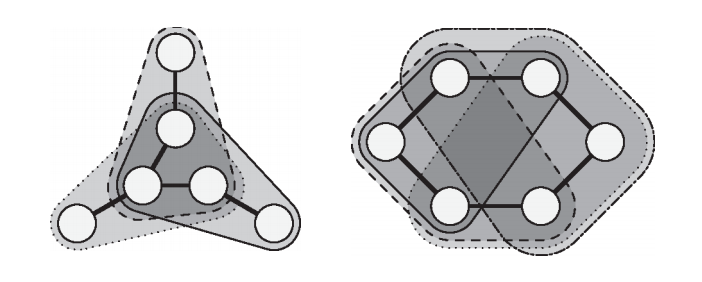
\includegraphics[width=\textwidth]{optimal-hypergraphs}
\caption{Examples of minimum supports. The hypergraph is represented with white nodes as hypervertices and hyperedges as gray areas. The support is the graph with white nodes and black edges connecting white nodes. (Source: Chen et al. \cite{Chen2015}) }
\end{figure}


\subsection{Supports}
A \textbf{support} graph or \textbf{support} $S = (V_S, E_S)$ of a hypergraph $H = (V_H, E_H)$ is a graph with the same vertex set as $H$, ie. $V_S = V_H$, in which the subgraph $G_e = (e, E_S \cap e \times e)$ of $H$ induced by each hyperedge $e \in E$ is a connected graph. Recall that each hyperedge $e$ is a set of vertices. In other words, a support graph of a hypergraph is able to "support" each of the hyperedges by keeping all the hypervertices in a hyperedge connected.
A planar support of a hypergraph is a support that can be drawn without overlapping edges.\\

Figure 2 shows two examples of support graphs of hypergraphs. Whichever hyperedge (grey region enclosed by black curve) you look at, all the vertices in that hyperedge is connected. If you remove any edge (black line connecting the white vertices), not all induced subgraphs of hyperedges are connected. Thus these are examples of minimal supports. In fact, they are minimum supports for the given hypergraphs.


\subsection{Problem Statement}
Thus our problem can be formally stated as:\\
For a given hypergraph, represented as a set of regions in a simple closed Jordan curve $\mathcal{R} = \{ R_1, ... , R_n \}$, build a planar graph $G$ on $R$ such that for each $p \in \mathbb{R}^2$, the set $\{R \in \mathcal{R} : p \in R\}$ forms a connected subgraph of $G$. 


Chen et al. \cite{Chen2015} gave an overview of the history and status quo of research around support graphs. They analyze multiple different research fields and concludes that the following problems that are the same problem of finding Supports of Hypergraphs:
\begin{enumerate}
\item Subset Interconnection Design Problem (SID)
\item Minimum Topic-Connected Overlay
\item Interconnection Graph Problem
\item Network Inference
\item Host graphs
\item Spanning graphs
\item Support (only certain structures)
\end{enumerate}
Such different names arose from different research fields  \cite{Chen2015}


\subsection{Specific Goals}

This research project will not aim at completely solving the problem of finding planar supports of hypergraphs but at solving several specific sub-problems that will help gain a greater understanding of the problem or novel ways to approach it.\\

Here I propose a few feasible sub-problems that this research project will attempt to solve.
\begin{enumerate}
\item Determine if 1-outer planar support exists for general hyperedges
\item Assuming that a planar support of a given hypergraph exists, how can we efficiently find an approximation such as a $k$-planar graph? 
\item Find a planar support of a hypergraph where the shapes of the regions are restricted to rectangles, disks, or arbitrary shapes that have at most $k$ number of intersections with other regions.
\item Given k-piercing regions (defined as regions pierced by maximum or on average k other regions), can we find a planar support?
\item Continue on Chen et al.'s work of varying the following parameters: 
size $d$ of the largest hyperedge, 
number $m$ of hyperedges in hypergraph,
feedback edge number $\phi = k-n+1$ of the solution -- this is a measure of sparseness where $k=$ number of edges in the solution and $n=$ number of vertices in original hypergraph.
\end{enumerate}

% Your Literature Review
\subsection{Related Work}
% Give an overview of the current state of knowledge on the particular topics. Include competing ideas and hypotheses as well as the major lines of evidence supporting or not supporting the different hypotheses. 
%Describe related work. All citations in your bibliography must be referenced in your proposal.

Johnson and Pollak proved that it is NP-complete to decide if a given hypergraph has a planar support.
Buchin et al. proved that it is NP-complete to decide whether a hypergraph has a 2-outerplanar support and that it is NP-hard to decide if a hypergraph has a 3-outerplanar support. \cite{buchin2010}
% (A k-outerplanar graph is a graph that can be drawn in the plane without crossing such that after k-fold removal of the vertices on the outer-face there are no vertices left. https://www.sciencedirect.com/science/article/pii/S0166218X1400434X)

In contrast, there are polynomial time algorithms to test whether a given hypergraph has a planar support that is a path, cycle, or tree. \cite{johnson1987}
Ray proved that for non piercing regions there is always a planar support and the proof provides an algorithm in $O(n^3)$ time complexity. \cite{Pyrga2008}
If the set of hyperedges is closed under intersections and differences, it can be decided in polynomial time whether the hypergraph has a planar or outerplanar support. \cite{brandes2011}

Finding the minimum support of special structures is also of interest in some fields.
It is known that finding the minimum weight support is NP-hard. \cite{Du1998}
There have been efforts to approximate minimum support using genetic algorithms \cite{abuali1996} and polynomial time greedy algorithms. \cite{Du1998}

Under certain circumstances, the minimum support can be found in polynomial time.
A minimum weighted tree support can be computed in polynomial time. \cite{Korach2003} Buchin et al. also showed that a support with the minimum number of edges can be computed in polynomial time if the hypergraph is closed under intersections. \cite{buchin2010}


\subsection{Potential Impact}
% Describe why the proposed research is important.
% Provide a statement of what you think the impact of your research will be. Be as specific as possible. 

The goal of this research project is to contribute to the ongoing theoretical discussion of planar supports and is not necessarily motivated by applications. However, there exist multiple uses of the outcome of this research project, especially in visualizing big sets \cite{meulemans2013} or colored graphs \cite{hurtado2017}. In some cases, supports are used for Social Network Theory.

It is also a subproblem of the NP-hard Subset Interconnection Design problem, also known as Minimum Topic-Connected Overlay. This problem has many applications in design of scalable overlay networks, vacuum systems, reconfigurable interconnection network, etc. \cite{Chen2015}



\subsection{Methodology}
% Describe the approach and methodology you want to pursue in order to achieve the capstone goal and/or answer the research question.

This research will generally consist of iteration of the following process. Visualize the problem. Find mathematical proofs. Provide experimental evidence via programming. Branch the problem into more easily solvable problems. 

Depending on the nature of a sub-problem, I will also employ software to brute-force solutions or to create visual representations of hypergraphs and their supports in the different methods noted above.



\renewcommand\refname{References}
\bibliography{references}
% The IEEE bibliography style is NOT rBibliography listing all cited references.
% Feel free to use whatever style you prefer
\bibliographystyle{IEEEtran}

\end{document}

